% !TEX root = ../Main.tex
When operating a fusion reactor a continous process of diagnostics are necessary in order to optimise the plasma for the fusion process. One of the active diagnostic methods are interferometry.
The goal here is to measure the plasma electron density in the Danish Tokamak Undertaking reactor.
Using a interferometer one can measure the electron density \(n_e\) of the plasma. The refractive index of electromagnetic waves depend on the electron density and plasma frequency \(\omega_p\) as such:
\begin{align}
	\omega_p^2 \propto n_e
\end{align}
For O-mode plasma waves the refractive index is:
\begin{align}
	N_{\mathrm{O}} = \sqrt{1-\frac{\omega_p^2}{\omega^2}}
\end{align}
with \(\omega\) being the probing wave frequency.
The plasma will reflect the beam if the plasma frequency is larger than the beam frequency so
\begin{align}
	\omega > \omega_p = \sqrt{n_e\frac{e^2}{\epsilon_0 m_{e0}}}
\end{align}
Therefore the critical electron density becomes
\begin{align}
	n_e < n_c      & = \omega^2\frac{\epsilon_0\cdot m_{e0}}{e^2} \label{nenc} \\
	               & \qq*{which gives} \nonumber                               \\
	N_{\mathrm{O}} & = \sqrt{1-\frac{n_e}{n_c}}\label{NO}
\end{align}
With a probing frequency much higher than the plasma frequency and the critical density much higher than the electron density \cref{NO} can be approximated by:
\begin{align}
	N_{\mathrm{O}} & = \sqrt{1-\frac{n_e}{n_c}} \approx 1-\frac{1}{2}\frac{n_e}{n_c} 0 1-\frac{\omega_p^2}{2\omega^2}
\end{align}
With sufficient accuracy, the linear dependence of the O-mode refractive index on the electron density is obtained if the normalised quantities obey:
\begin{align}
	\frac{n_e}{n_c} \leq 0.4 \quad \frac{\omega_p}{\omega} \leq 0.6
\end{align}
We must calculate the phase shift as one beam travels in vacuum by the length \(L_V\) and one wave travels in the plasma by the length \(L_P\). The phase shift in terms of \(2 \pi\) is equal to the optical difference divided by the wavelength. With the refractive index in vacuum, \(N_V=1\), this yields:
\begin{align}
	\frac{\Phi}{2\pi} & = \frac{\Delta L_{opt}}{\lambda} = \frac{\int_{x_1}^{x_2}\pqty{N_V-N_{\mathrm{O}}(x')}\dd{x'}}{\lambda} \approx \frac{1}{2\lambda n_c}\int_{0}^{x}n_e(x')\dd{x'} \\
	                  & = 4.48\times 10^{-16} \pqty{\frac{\lambda}{\si{\meter}}}\int_{0}^{x}\pqty{\frac{n_e(x')}{\si{\per\meter\cubed}}}\pqty{\frac{\dd{x'}}{\si{\meter}}}
\end{align}
Assuming a Gaussian distribution, the electron density at \(\pm\infty\) is approximately equal to the densities just inside the reactor walls. Therefore
\begin{align}
	\int_{-\infty}^{\infty}n_e \exp\pqty{-\frac{(y-b)^2}{2c^2}}\dd{y} \approx n_e\ c\ \sqrt{2\pi}\label{c}
\end{align}
With the density at the centre given as:
\begin{align}
	\SI{e16}{\per\meter\cubed} \leq n_e \leq \SI{e18}{\per\meter\cubed},
\end{align}
The \(c\) in \cref{c} is the width of the Gaussian distribution and must fit inside the reactor. The DTU tokamak has a minor diameter of \SI{0.25}{\meter}. Thus
\begin{align}
	\frac{\Phi(x)}{2\pi} \approx 4.48\times 10^{-16}\pqty{\frac{\lambda}{\si{\meter}}}\SI{0.25}{\meter}n_e & = 1.12\times 10^{-16}\ n_e \pqty{\frac{2\pi\ \SI{0.25}{\meter}}{\omega\si{\meter}}} \\
	                                                                                                       & = 1.12\times 10^{-16}\ n_e\pqty{\frac{2\pi\SI{3e8}{\per\second}}{\omega}}           \\
	                                                                                                       & = 2.1112\times 10^{-7}\pqty{\frac{n_e}{\omega\si{\second}}}
\end{align}
Remembering \cref{nenc}
\begin{align}
	\omega^2\frac{\epsilon_0\cdot m_{e0}}{e^2} & = \omega^2\frac{\SI{8.854e-12}{\farad\per\meter}\SI{9.109e-31}{\kilo\gram}}{\SI{1.602e-19}{\coulomb}} \\
	                                           & \Downarrow\nonumber                                                                                   \\
	n_e                                        & < 0.000314\omega^2 \label{co}
\end{align}
Where any units has been disregarded. We want the largest possible phase shift which means that the lower the frequency the better. However cutoff must first be taken into account.
Since the cutoff is given by \cref{co} and since we want to measure densities up to \SI{e18}{\per\meter\cubed} the minimum frequency of the wave is
\begin{align}
	\frac{\omega}{2\pi} & > \frac{\sqrt{\frac{\SI{e18}{\per\meter\cubed}}{0.000314}}}{2\pi} \\
	                    & \Downarrow\nonumber                                               \\
	f                   & \approx \SI{9}{\giga\hertz}
\end{align}
Given the available emitters, the best emitter is therefore the one with $f=60\si{GHz}$.

\subsection{Evolving beam width}

\subsection{Gauss telescope arrangement}
From chapter 5 in ``Fusion Plasma Diagnostics with mm-Waves''\cite{PlasmaDiagnosis} the authors argue that a Gauss telescope arrangement can alter the beam waist independently of wavelength. This motivates narrowing the interferometer beam waist with a lense system.
\begin{figure}
    \centering
    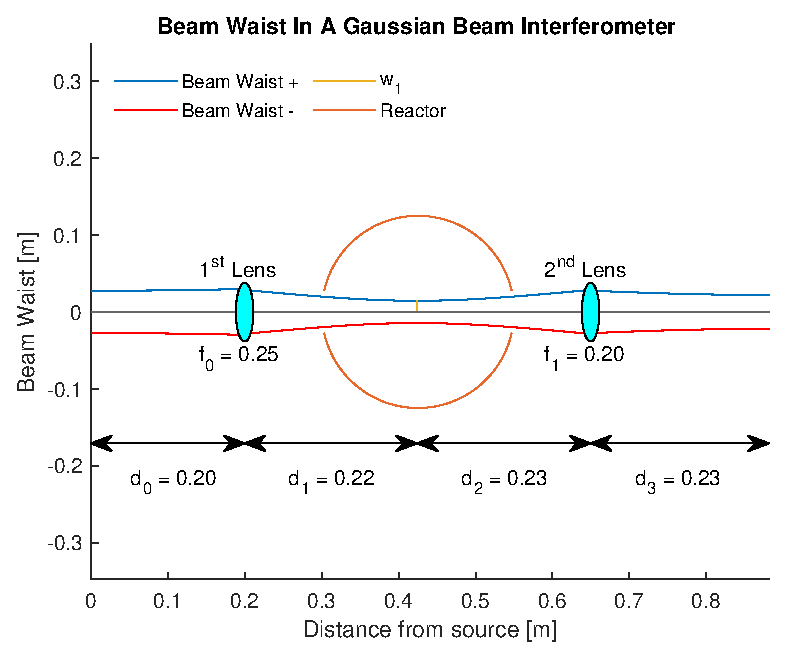
\includegraphics[width=.9\textwidth]{MatlabFigures/Interferometer/Interferometer.eps}
    \caption{Awesome Gaussian Telescope}
    \label{AWESOME}
\end{figure}